\documentclass[10pt]{article}
\usepackage[
    backend=biber,
    style=numeric,
]{biblatex}
\usepackage{graphicx}
\usepackage{caption}
\usepackage{subcaption}

% Page settings
\usepackage[top=1in, bottom=1in, left=1in, right=1in, centering]{geometry}

% Macros
% Macros for entire document

% Utility commands
\newcommand{\bc}{\begin{center}}
\newcommand{\ec}{\end{center}}
\newcommand{\beq}{\begin{equation}}
\newcommand{\eeq}{\end{equation}}
\newcommand{\bea}{\begin{eqnarray}}
\newcommand{\eea}{\end{eqnarray}}
\newcommand{\ba}{\begin{array}}
\newcommand{\ea}{\end{array}}

% Fancy equation environments
\newcommand{\Eq}[2][Eq.~]{{#1}(\ref{eq:#2})}                                    
\newcommand{\Eqs}[1]{Eqs.~(\ref{eq:#1})}                                        
\newcommand{\Fig}[2][Fig.~]{{#1}\ref{fig:#2}}                                   
\newcommand{\Figs}[1]{Figs.~\ref{fig:#1}}                                       
\newcommand{\Sec}[2][Sec.~]{{#1}\ref{sec:#2}}                                   
\newcommand{\Secs}[1]{Secs.~\ref{sec:#1}}      

% Common expressions
\def\eg{\emph{e.g.}}
\def\ie{\emph{i.e.}}
\def\etal{\emph{et al.}}
\def\etc{\emph{etc.}}

% Mathematical notation
\def\cross{\ensuremath{\times}}
\def\div{\ensuremath{\nabla \cdot}}
\def\divs{\ensuremath{\nabla_{s} \cdot}}
\def\grad{\ensuremath{\nabla}}
\def\grads{\ensuremath{\nabla_{s}}}
\def\lapl{\ensuremath{\nabla^2}}
\newcommand{\tensor}[1]{\ensuremath{{\bf{#1}}}}
\newcommand{\vectornorm}[1]{\left|\left|#1\right|\right|}

\newcommand{\ddx}[2]{\frac{d#1}{d#2}}
\newcommand{\DDx}[2]{\frac{\partial #1}{\partial #2}}
\newcommand{\sgn}[1]{\ensuremath{\mathrm{sgn}(#1)}}
\newcommand{\abs}[1]{\ensuremath{\left|#1\right|}}

% Code
\newcommand{\code}{\texttt}


% Resources
\graphicspath{{figures/}}
\addbibresource{single-sensor-ica-for-moving-sources.bib}

\title{
    Investigation of Independent Component Analysis (ICA) for
    Single-Sensor Hydrophone Recordings of Moving Sources
}

\author{
Prepared for IQTLabs \\
by Kevin Chu \\
Velexi Corporation
}

\date{Version: 1.1\\(March 20, 2023)}

\begin{document}

\maketitle

\abstract{
The performance of any machine learning system depends critically on the quality of the
input features. For signals processing applications, independent component analysis (ICA)
is one method that can be used to develop features that are
tuned to the application by extracting source signals that are statistically
independent from each other. While ICA classically requires multiple sensors that
simultaneously record data, ICA can, under certain circumstances, be applied to
single-sensor systems by using \emph{recordings at multiple times}. In this report, we
leverage the physics of acoustic waves to develop ICA approaches that are suitable for
single-sensor systems when sources are moving relative to the sensor and each other.
Consistent with the quasi-periodic nature of the source signals, we find that the
theoretically most promising approach for source separation is ICA performed in the
frequency-domain. Using synthetic datasets constructed from pure source audio clips, we
evaluated the performance of all approaches except for the most promising one (because,
unfortunately, readily-available implementations of the FastICA algorithm are currently
unable able to handle complex-valued data). We assessed all approaches by comparing the
power spectra of source signals estimated by ICA against the power spectra of ground truth
pure source signals. The results of the computational experiments were found to be
consistent with theoretical expectations.

\paragraph{Key Technical Outcomes}
\begin{itemize}
    \item Development of an ICA approach that is suitable for single-sensor systems when
        sources are in motion.

    \item Theoretical analysis of ICA-based approaches to source separation for source
        signals that are phase-synchronized and phase-unaligned across multiple recording
        times.

    \item Use of power spectra to characterize quasi-periodic source signals and assess
        the quality of ICA estimates for source signals.

    \item Validation of theoretical expectations for ICA-based approaches via computational
        experiments.

    \item Identification of potential key obstacle to a robust ICA approach for separating
        quasi-periodic source signals.
\end{itemize}

}


\section{Introduction}
Independent Component Analysis (ICA) is a technique for extracting independent source
signals from measurements of mixtures of the source signals~\cite{sklearn-bss,
hyvarinen:2000,tharwat:2021}. It is commonly used in situations where there are multiple
sensors simultaneously collecting measurements for sources whose characteristics (\eg,
location) do not change over time. For situations where there is only a single sensor, ICA
may still be viable if (1) the sources are moving (relative to the sensor and each other),
(2) it is performed on multiple signal clips recorded at different times, and (3) the
assumptions of the ICA model are valid for the mixed signal clips.

\subsection*{ICA Source Signals as ML Features}
ICA can be useful as a feature engineering method. The source signals estimated by ICA
(possibly across mulitple non-overlapping applications of ICA) define a dictionary of
potential source signals. Methods, such as simple orthogonal projection or sparse
approximation~\cite{blumensath:2009,needell:2009,wikipedia-sparse-approximation}, can be
used to convert unknown signals into a set of features that are likely to be related to
the types of sources present. In a sense, these ICA features are more likely to be
\emph{tuned} for the identification of sources and should, in principle, simplify the
mappings that any ML algorithm needs to learn in order to perform well.

\subsection*{Quasi-Periodic Source Signals}
In the approaches described in this report, we leverage an observation about the source
signals of interest: they are quasi-periodic --- that is, they are qualitatively but not
necessarily precisely repetitive. Mathematically, source signals with this quality have
\emph{temporally stable power spectra}. In the following development, this stability of the
power spectra is used for both (1) the development of ICA approaches for source separation
and (2) the assessment of ICA performance. Figure~\ref{fig:power-spectra-examples} shows
example power spectra of hydrophone recordings from individual vessels.
\begin{figure}[ht]
    \centering
    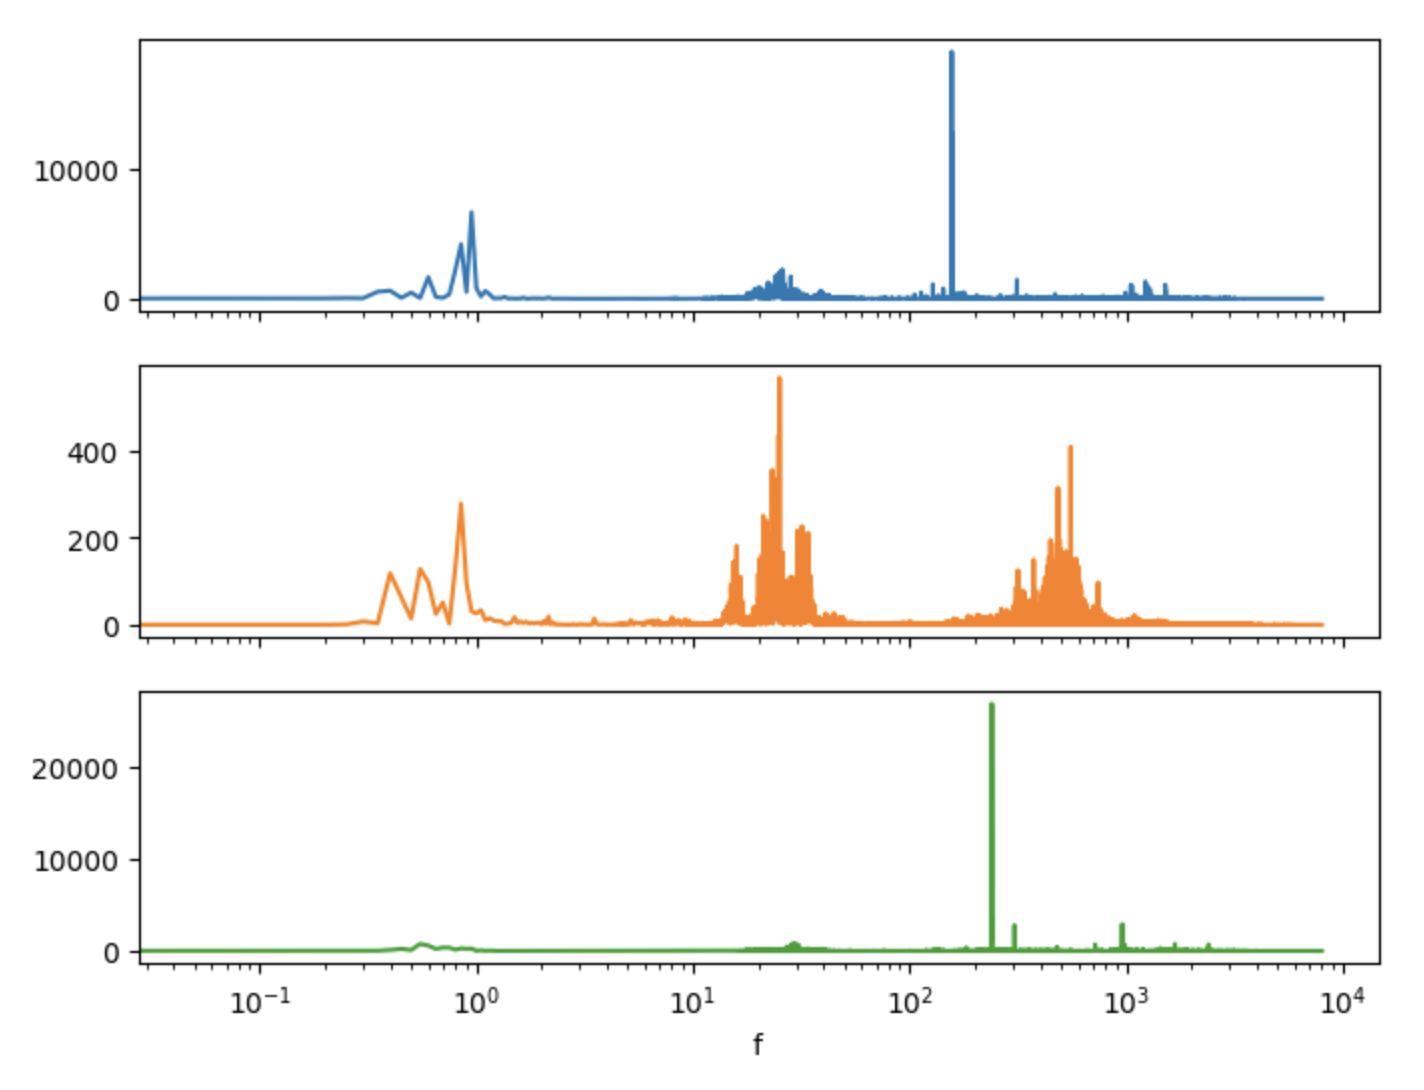
\includegraphics[width=0.5\textwidth]{power-spectra-examples}
    \caption{\label{fig:power-spectra-examples}
        Example power spectra of hydrophone recordings from individual vessels.
    }
\end{figure}

\subsection*{Organization of Report}
In this report, we investigate the use of ICA for separation of source signals in
single-hydrophone recordings of sources that are in motion relative to the hydrophone and
each other. We begin with a brief review of basic ICA theory and its application when
multiple sensors are used for recording. Second, we present an approach for using ICA when
only a single sensor is available by recording clips at multiple times. Next, through
controlled computational experiments using synthetic datasets, we probe the conditions
required to achieve useful signal separation. Finally, we summarize our findings and
comment on promising directions for future research and development.

\subsection*{Notation and Abbreviations}
\begin{itemize}
    \item DFT: discrete Fourier transform
    \item ICA: independent component analysis
\end{itemize}


\section{ICA Foundations}
Independent component analysis is a technique that estimates statistically independent
source signals from mixed signals. It is one of several approaches for performing
\emph{blind source separation}. In this section, we present the ICA signal model and
describe its use for source separation in the classical case when multiple sensors are
used to collect measurements.

\subsection*{Signal Model}
In ICA, each mixture signal $s_i(t)$ is assumed to be a linear combination of the source
signals:

$$
s_i(t) = \sum_{j=1}^N a_{ij} x_j(t)
$$

\noindent where $s_i(t)$ is the $i$-th mixed signal, $x_j(t)$ is the $j$-th source signal,
and $a_{ij}$ is the contribution of the $j$-th source to the measurement at the $i$-th
sensor. Because the $a_{ij}$ define how the source signals are mixed to obtain the sensor
signals, they are called \emph{mixing coefficients}. The mixing equations can be expressed
in matrix form as:

$$
\vec{s}(t) = \mathbf{A} \vec{x}(t)
$$

\noindent where $\vec{s}(t) =  (s_1(t), \ldots, s_M(t))^T$ and
$\vec{x}(t) =  (x_1(t), \ldots, x_M(t))^T$
are the sensor and source signal vectors, respectively, and $\mathbf{A}$ is the
\emph{mixing matrix}. In general, up to $M$ source signals can be estimated when $M$ mixed
signals are available for analysis.

In a noisy environment, the signal model is modified to include a noise term

$$
s_i(t) = \sum_{j=1}^N a_{ij} x_j(t) + \sigma w_i(t)
$$

\noindent where $w_i(t)$ is Gaussian white noise with power $\sigma^2$.

\subsection*{FastICA}
There are several algorithms for solving the ICA equations. The implementation that is
readily available in the \code{scikit-learn} Python is based on
FastICA~\cite{hyvarinen:1999, sklearn-fastica}, an algorithm that uses fast fixed-point
iteration to simultaneously solve for the source signals $x_j(t)$ and the mixing
coefficients $a_{ij}$. It is important to note that the FastICA implementation available
in \code{scikit-learn} only supports real-valued data. Unfortunately, this contraint limits
our ability to assess the utility of ICA in situation where it would be beneficial to
perform ICA on the Fourier transform of the raw signal.

\subsection*{Classical Application of ICA: Multi-Sensor Systems}
ICA is most commonly applied to time-series data gathered by making measurements with
\emph{multiple, synchronized} sensors. For these types of systems, the data is real-valued
(because we are able to analyze the data in the time domain), so it is straightforward to
perform ICA using the FastICA implementation available in \code{scikit-learn}.
Figure~\ref{fig:multi-sensor-ica} illustrates the use of ICA on multi-sensor,
time-synchronized data.

\begin{figure}[ht]
    \centering
    \hspace{-0.25in}
    \begin{subfigure}{0.3\textwidth}
        \centerline{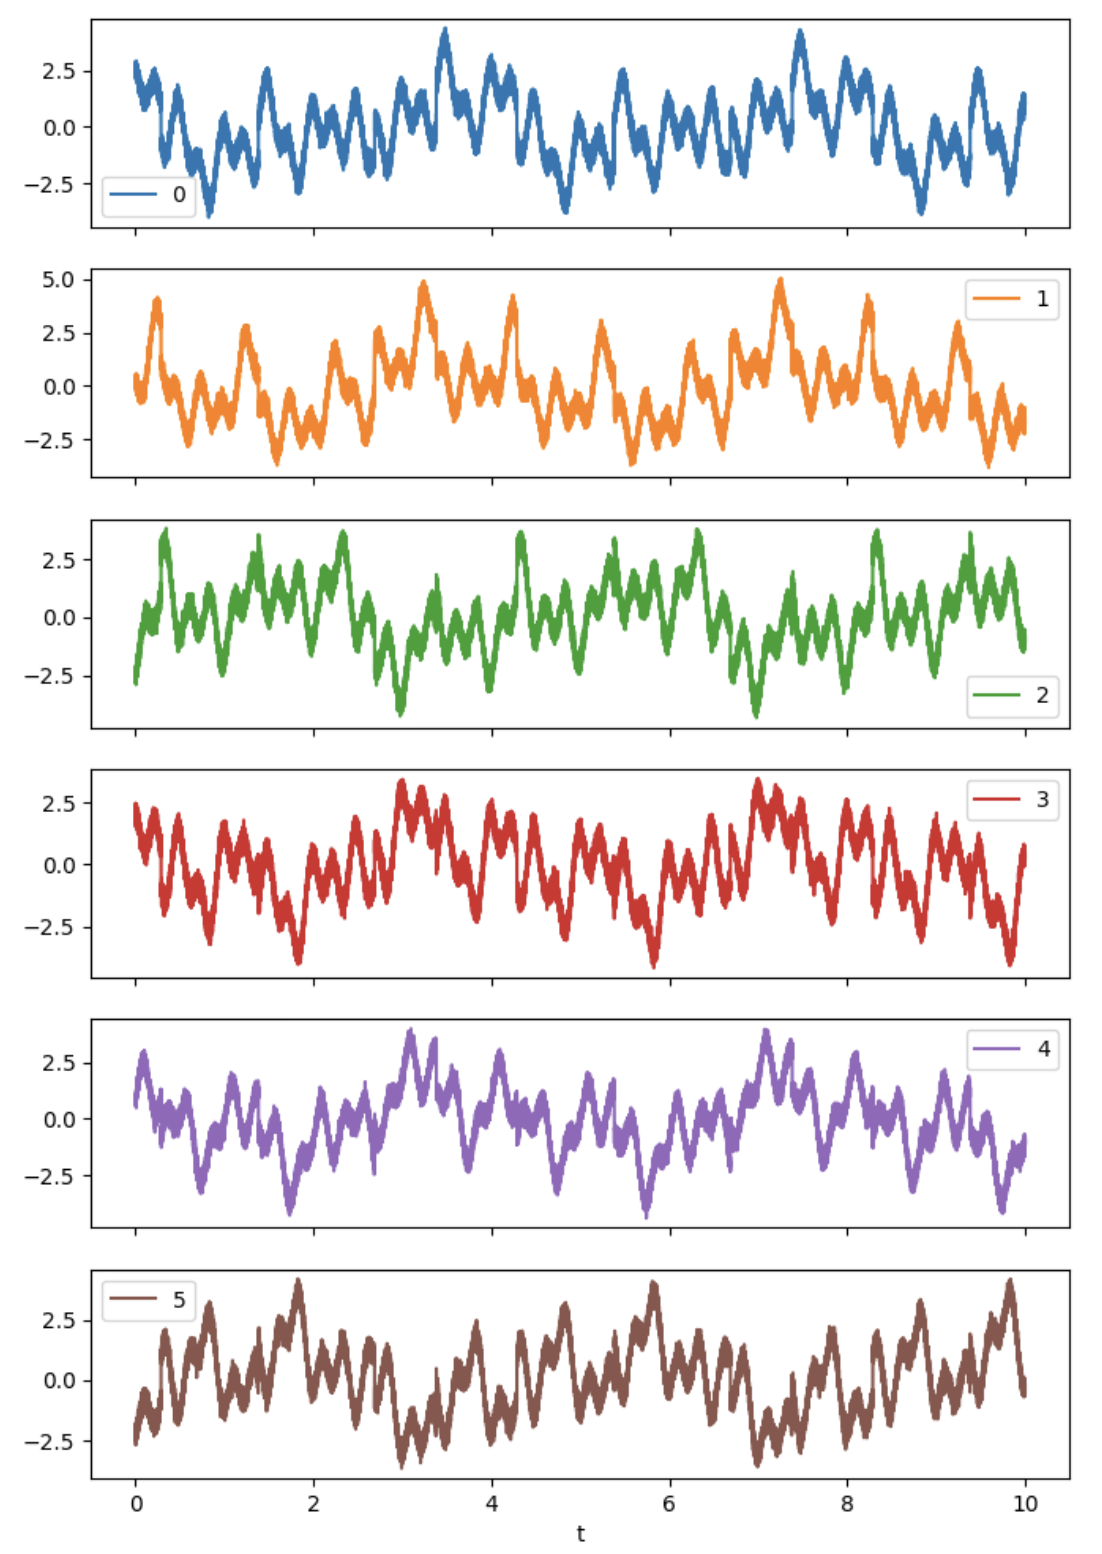
\includegraphics[height=2.3in]{multi-sensor-ica-mixed-signals}}
        \caption{}
    \end{subfigure}
    \begin{subfigure}{0.3\textwidth}
        \centerline{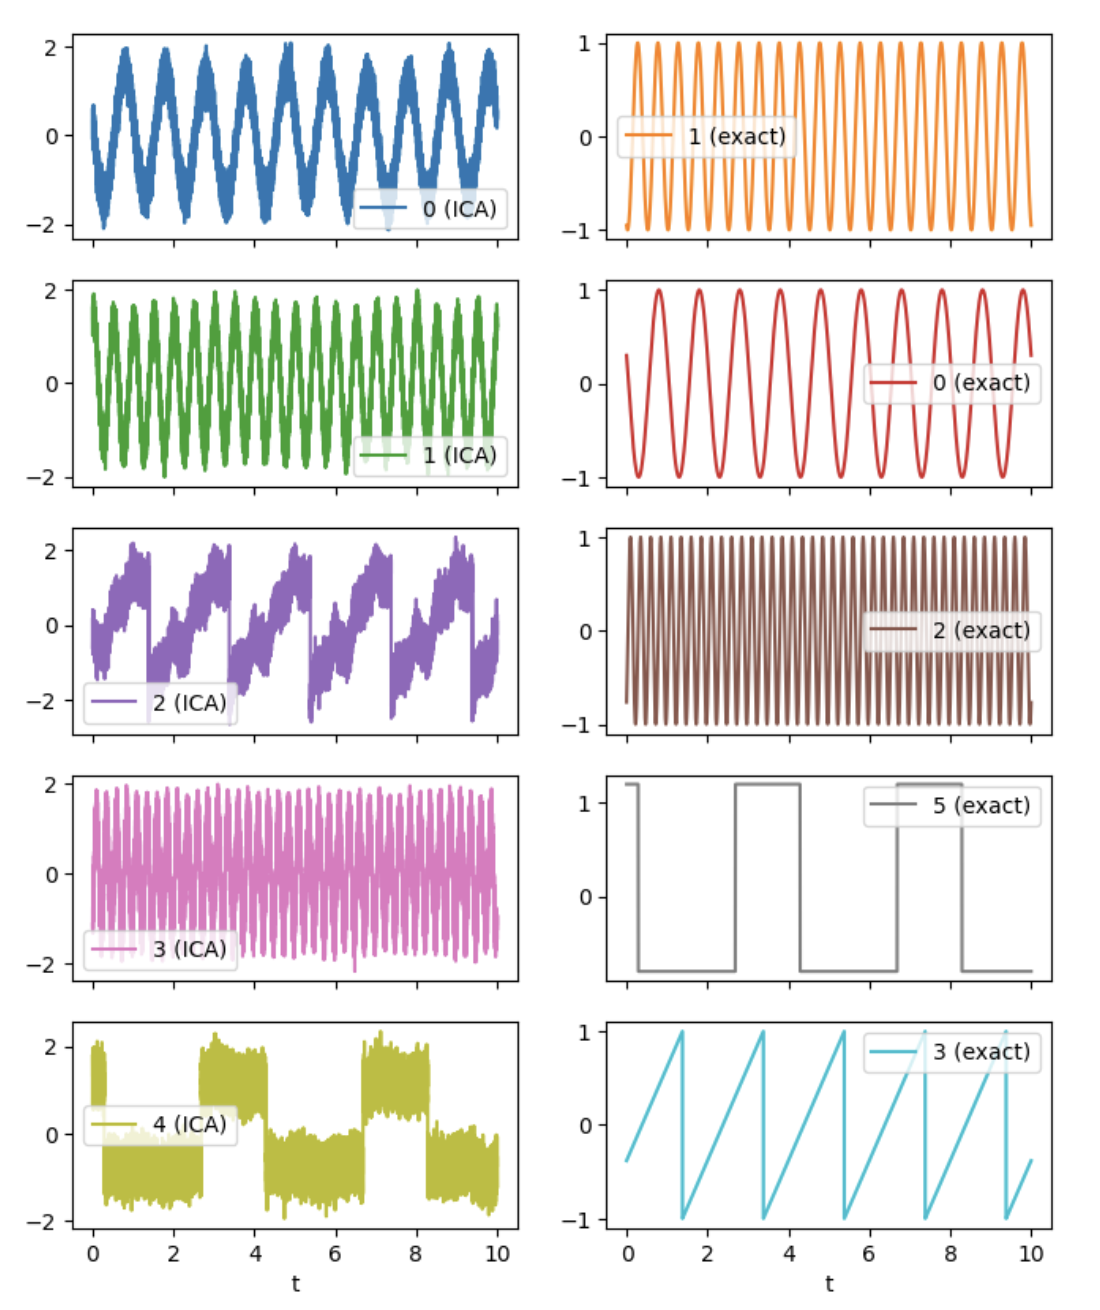
\includegraphics[height=2.3in]{multi-sensor-ica-source-signals}}
        \caption{}
    \end{subfigure}
    \begin{subfigure}{0.3\textwidth}
        \centerline{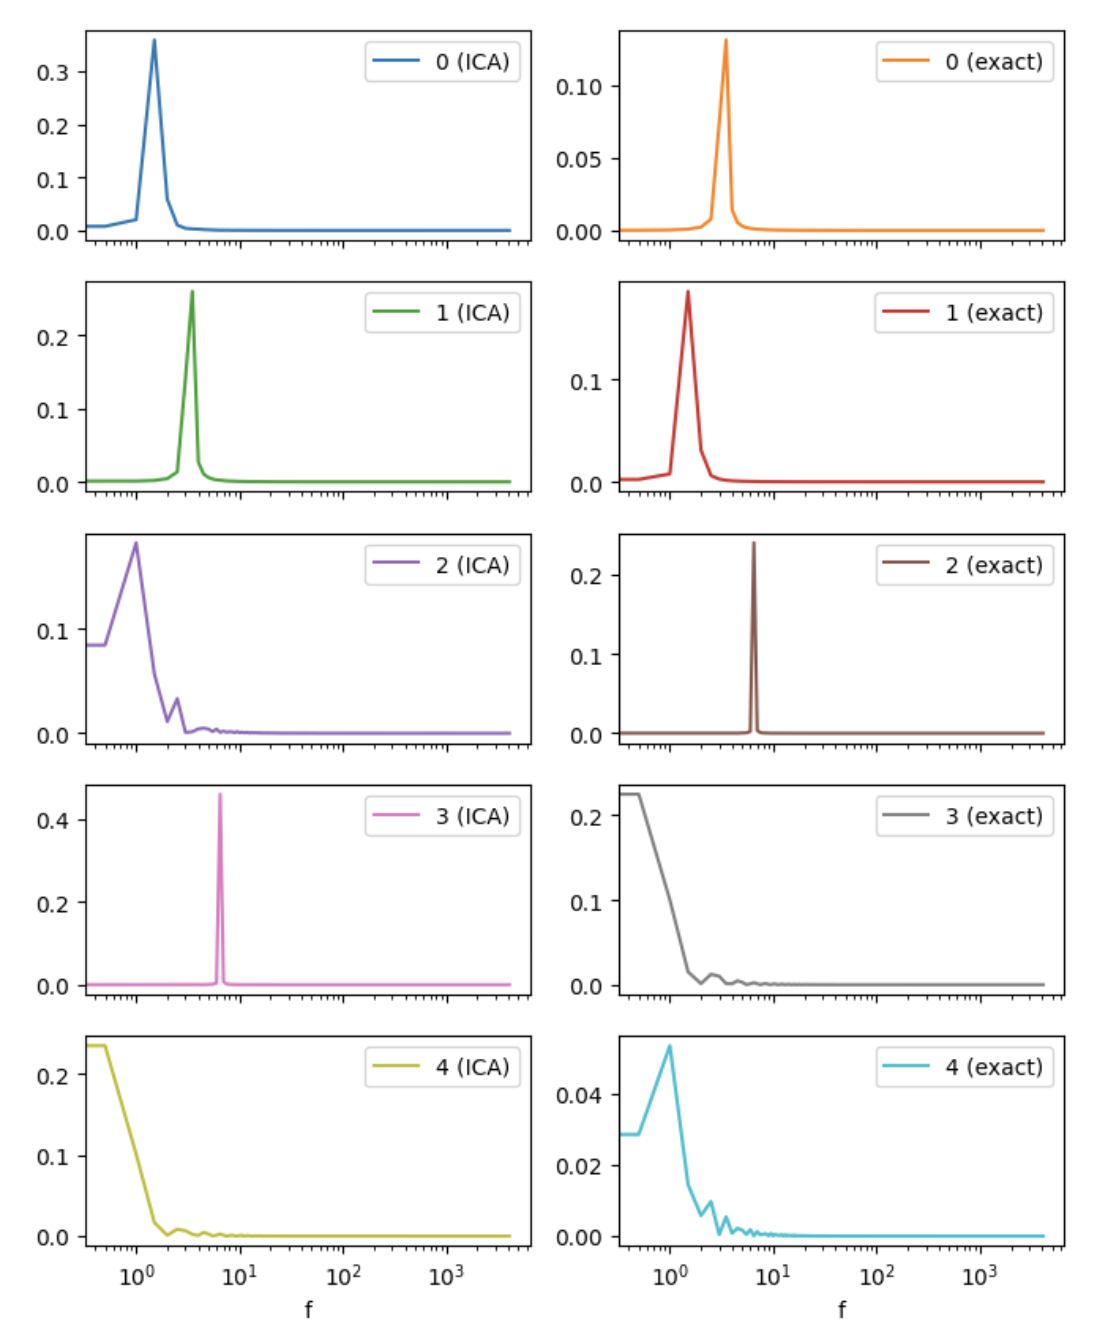
\includegraphics[height=2.3in]{multi-sensor-ica-source-power-spectra}}
        \caption{}
    \end{subfigure}

    \vspace{0.1in}
    \begin{minipage}{0.85\linewidth}
    \caption{\label{fig:multi-sensor-ica}
        ICA applied to the classical source separation problem with multiple sensors
        simultaneously making measurements.
        (a)~Mixed signals measured simultaneously by five different sensors.
        (b)~Source signals in the time domain: extracted via ICA (left) and ground truth
        (right).
        (c)~Power spectra of source signals: extracted via ICA (left) and ground truth
        (right).
    }
    \end{minipage}
\end{figure}


\section{ICA For Moving Sources Using Single-Sensor Recordings}
When sources are in motion relative to each other, it is theoretically possible to use ICA
for source separation with only a single sensor by \emph{collecting recording clips at
multiple times} as long as three conditions are met:
\begin{itemize}
    \item at each time, the recording is a linear combination of source signals,

    \item the source signals are synchronized in the domain that ICA is performed in
        (\ie, time or frequency), and

    \item the coefficients used to combine source signals change non-trivially between
        recording times.
\end{itemize}
For sound waves, the first and third conditions are satisified under weak assumptions.
The second condition, however, requires stronger assumptions.

Under the weak assumption that wave propogation is well-modeled by the linear wave equation,
the origin of the first condition is the principle of superposition for the wave equation
--- the pressure at the sensor location is a linear combination of the pressure waves from
each of the sources. Note that the condition is satisfied in both the time and frequency
domains.

The third condition holds because pressure is proportional to the inverse of the distance
between the source and sensor. As a result, the relative magnitudes of the contribution of
sources changes between recording times (assuming the time interval between recordings is
sufficiently large for sources to have moved a significant distance). Note that while there
are source trajectories that would cause the relative magnitudes of the pressure to remain
constant, these motions are atypical.

The second condition is only satisfied under special assumptions. In the time domain, the
second condition only holds if the relative phases of source signals are synchronized
across recordings --- in other words, the relative phase of the source signals is the same
for all signals at all recording times. When this condition is met, ICA can be used to
perform source separation in the time domain. Unfortunately, this condition unlikely to be
met because sources typically have different periodicities, so source phases are do not
remain aligned in time. Since recording times are chosen without knowledge of the sources,
it is unlikely that they would happen to be chosen such that source phases are aligned
across recordings.

When unaligned source signal phase shifts are present between recordings, the signal model
becomes
$$
s_i(t) = \sum_{j=1}^N a_{ij} x_j(t + \phi_{ij}),
$$
and ICA is not directly applicable to the time-domain signal. In this situation, it is
useful to use the Fourier transform to convert signals to the frequency domain because
phase shifts in the time domain become multiplication by a complex exponential in the
frequency domain. For this approach to be viable, we require two additional assumptions
--- one for the type of Fourier analysis and one for the structure of the source signals.
\begin{itemize}
    \item The Fourier transform must be performed using the complex exponential Fourier
        basis. When sines and cosines are used as basis functions, phase shifts in time
        manifest as mixing between the coefficients of the basis functions which is
        incompatible with the signal model for ICA.

    \item The source signals must be qualitatively repetitive so that the Fourier
        spectra of the source signals remains stable across all recordings.
\end{itemize}
When both of these conditions are met, the signal model in the \emph{frequency domain} is
$$
\hat{s}_i(f) = \sum_{j=1}^N a_{ij} \hat{x}_j(f),
$$
where $\hat{s}_i(f)$ and $\hat{x}(f)$ are the Fourier transforms of $s_i(t)$ and $x(t)$,
respectively, and $a_{ij}$ are mixing coefficients that \emph{implicitly encode the
relative phase shifts between source signals}. This equation has the same form as the ICA
signal model, so source separation can be achieved by applying ICA in the frequency domain.
It is important, however, to emphasize that in this model, all quantities are
\emph{complex-valued}.

\section{Computational Experiments}

To evaluate the effectiveness of and failure cases for source separation using ICA, we
performed a series of computational experiments:
\begin{itemize}
    \item ICA on time-domain signals when source signals are phase-synchronized across
        recording times;
    \item ICA on time-domain signals when relative phase shifts are present between source
        signals at different recording times; and
    \item ICA on frequency-domain signals using a sine and cosine basis when relative phase
        shifts exist between source signal.
\end{itemize}
Unfortunately, due to limitations of the FastICA implementation in \code{scikit-learn}, we
were unable to perform a computational experiment for the most promising approach for
source separation in the presence of relative phase shifts between source signals: ICA on
frequency-domain signals using a complex exponential basis.

\subsection*{Methodology}
Each experiment was performed using the following procedure. Each of these steps is
described in more detail its own subsection.

\begin{enumerate}
    \item Generate a synthetic dataset of mixed signals from recordings of individual
        sources.

    \item Preprocess the mixed signals to extract segments to use as input to ICA.

    \item Perform ICA on the preprocessed mixed signals.

    \item Assess the quality of source separation by qualitatively comparing the power
        spectra of estimated and ground truth source signals. \emph{Note}: unlike the
        simple demonstration presented for classical ICA, the complexity of the source
        signals precludes direct comparison in the time domain.
\end{enumerate}

\subsubsection*{Dataset Generation}
For each experiment, we constructed a synthetic dataset by combining audio clips for pure
sources in the following manner (for more details, see the help message for the
\code{generate-synthetic-dataset.py} script).

\begin{itemize}
    \item First, we select random initial positions (relative to the sensor) for all of
        the sources. If distances from the pure sources are known, those distances are
        used; otherwise, source distances are selected randomly. Azimuths for all sources
        are randomly selected.

    \item Next, we randomly select the heading and velocity for each source.

    \item At multiple recording start times that allow for the sources to travel far
        enough to change the strength of their signals at the sensor, we use the
        theoretical solution to the pressure wave equation to estimate the signal strength
        for each source.

    \item For experiments where there are relative phase shifts between source signals,
        a random temporal shift is selected for each source signal at each recording time.

    \item For each recodring time, a mixed signal recording is constructed by combining
        the pure source signals with (1) scaling implied by the estimated signal
        strength at the new source position and (2) a temporal shift (if applicable).
\end{itemize}

\subsubsection*{Signal Preprocessing}
Before performing ICA, each recording is preprocessed using the following procedure.

\begin{itemize}
    \item We performed experiments with and without bandpass filtering of the raw mixed
        signal. Our hypothesis was that bandpass filtering to remove low and
        high frequencies likely to have strong non-source contributions (\eg, wind noise)
        would improve ICA performance. When bandpass was applied, we used a Butterworth
        filter with the parameters:

        \begin{itemize}
            \item Passband: [5, 1000] Hz
            \item Stopband Edges: [1, 1500] Hz
            \item Maximum Loss in Passband (dB): 1
            \item Minimum Attenuation in the Stopband (dB): 100
        \end{itemize}

    \item A 20 second snippet of the recording is extracted for ICA. The duration of the
        snippet is chosen to be (1) short enough that the signal strength from sources
        does not change significantly during the snippet\footnote{Assuming a typical
        sensor-to-source distance of $500$m and a source speed of $1$m/s, the ratio of the
        pressure amplitude the source after $20$s of travel lies in the range $0.96$ to
        $1.04$.}, (2) long enough that the resolution of the discrete Fourier transform
        (DFT) of the signal is high enough to capture the structure of the power spectra of
        the source signals\footnote{For a $20$s sample, the spacing between frequencies in
        the DFT is $1 / 20 = 0.05$Hz, which for a $16$kHz sampling rate corresponds to a
        resolution of $(16000 / 2) / 0.05 = 160,000$ points for the power spectrum.}, and
        (3) long enough for a reasonably large number of ``quasi-cycles'' of the source
        signal to be included for analysis\footnote{Since the bandpass filter rejects
        frequencies below $5$Hz, a $20$s sample includes about 100 cycles of the lowest
        frequency for analysis.}.
\end{itemize}

\subsubsection*{ICA Analysis}
ICA was performed on the preprocessed audio snippets by using the \code{scikit-learn}
\code{FastICA} class with default parameters except for:
\begin{itemize}
    \item \code{n\_components}: set to the number sources to estimate
    \item \code{whiten}: set to \code{"unit-variance"}.
\end{itemize}


\subsubsection*{Evaluation of Source Signal Estimates}
To assess the quality of the source signals extracted by ICA, we visually compared the
power spectra of the estimated sources and the ground truth audio clips used to construct
the synthetic mixed signals.


\subsection*{Results and Discussion}

\subsubsection*{Time-Domain ICA For Phase-Synchronized Source Signals}
For source signals that are phase-synchronized across recording times, ICA was found to be
effective for estimating source signals from multiple, time-separated recordings collected
using a single, stationary sensor.
Figure \ref{fig:single-sensor-ica-time-domain-phase-synchronized-without-filter-source-power-spectra}
compares the power spectrum of the estimated and ground truth source signals
without bandpass filtering.
Figure~\ref{fig:single-sensor-ica-time-domain-phase-synchronized-with-filter-source-power-spectra}
compares the power spectrum of the estimated and ground truth source signals with bandpass
filtering.

\begin{figure}[ht]
    \centering
    \hspace{-0.25in}
    \begin{subfigure}{0.4\textwidth}
        \centerline{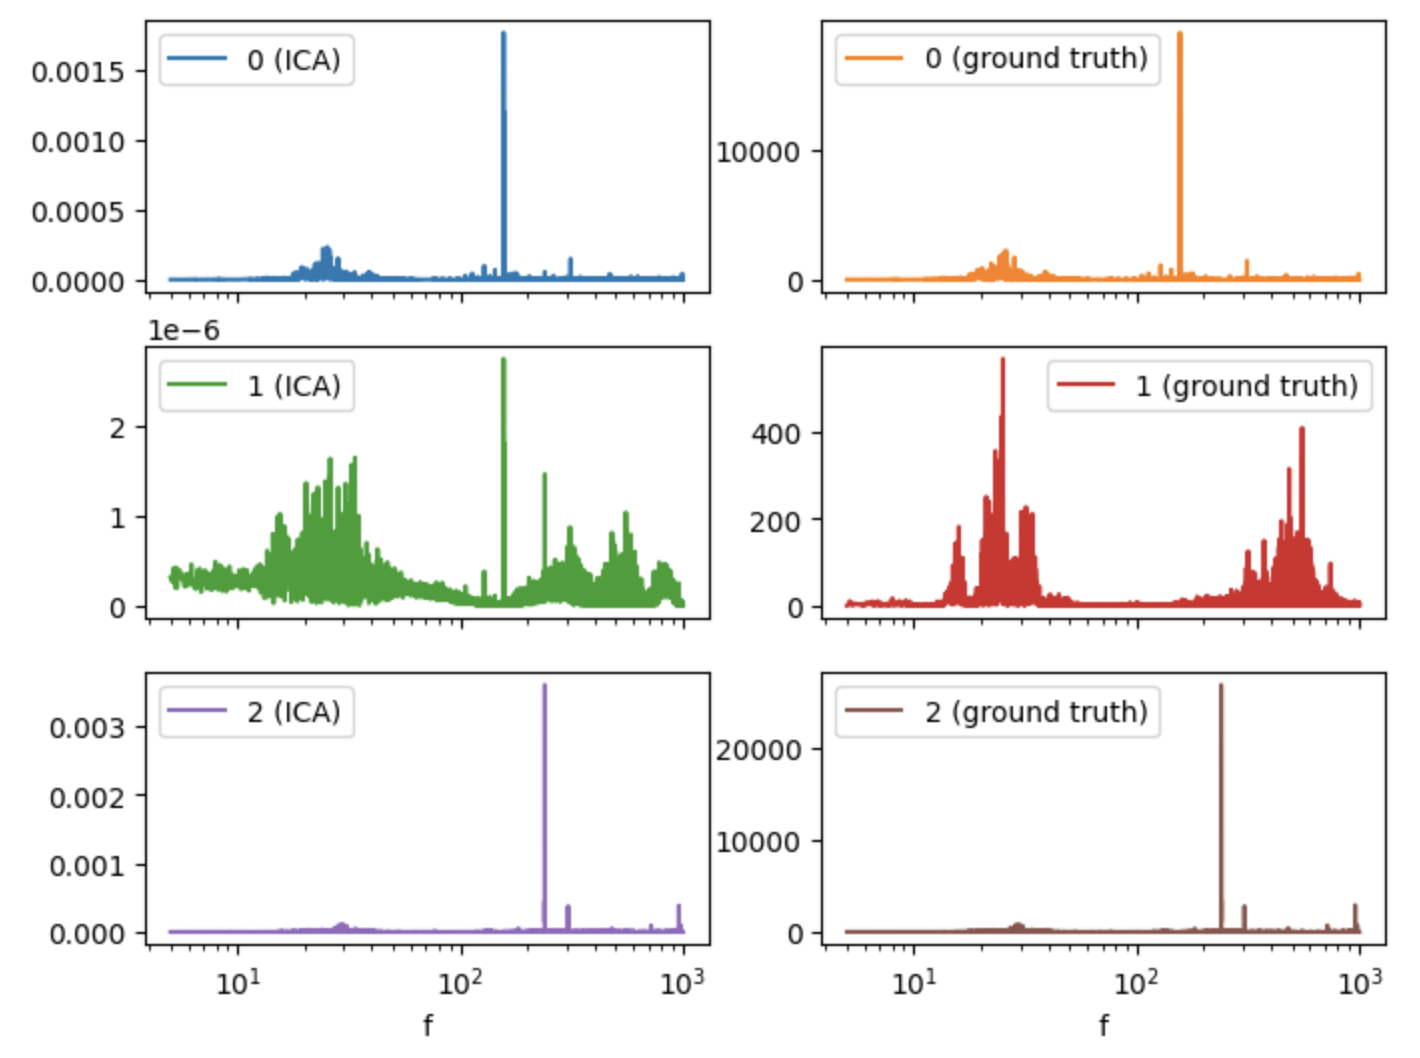
\includegraphics[width=\textwidth]{single-sensor-ica-time-domain-phase-synchronized-without-filter-source-power-spectra}}
        \caption{\label{fig:single-sensor-ica-time-domain-phase-synchronized-without-filter-source-power-spectra-passband}}
    \end{subfigure}
    \begin{subfigure}{0.4\textwidth}
        \centerline{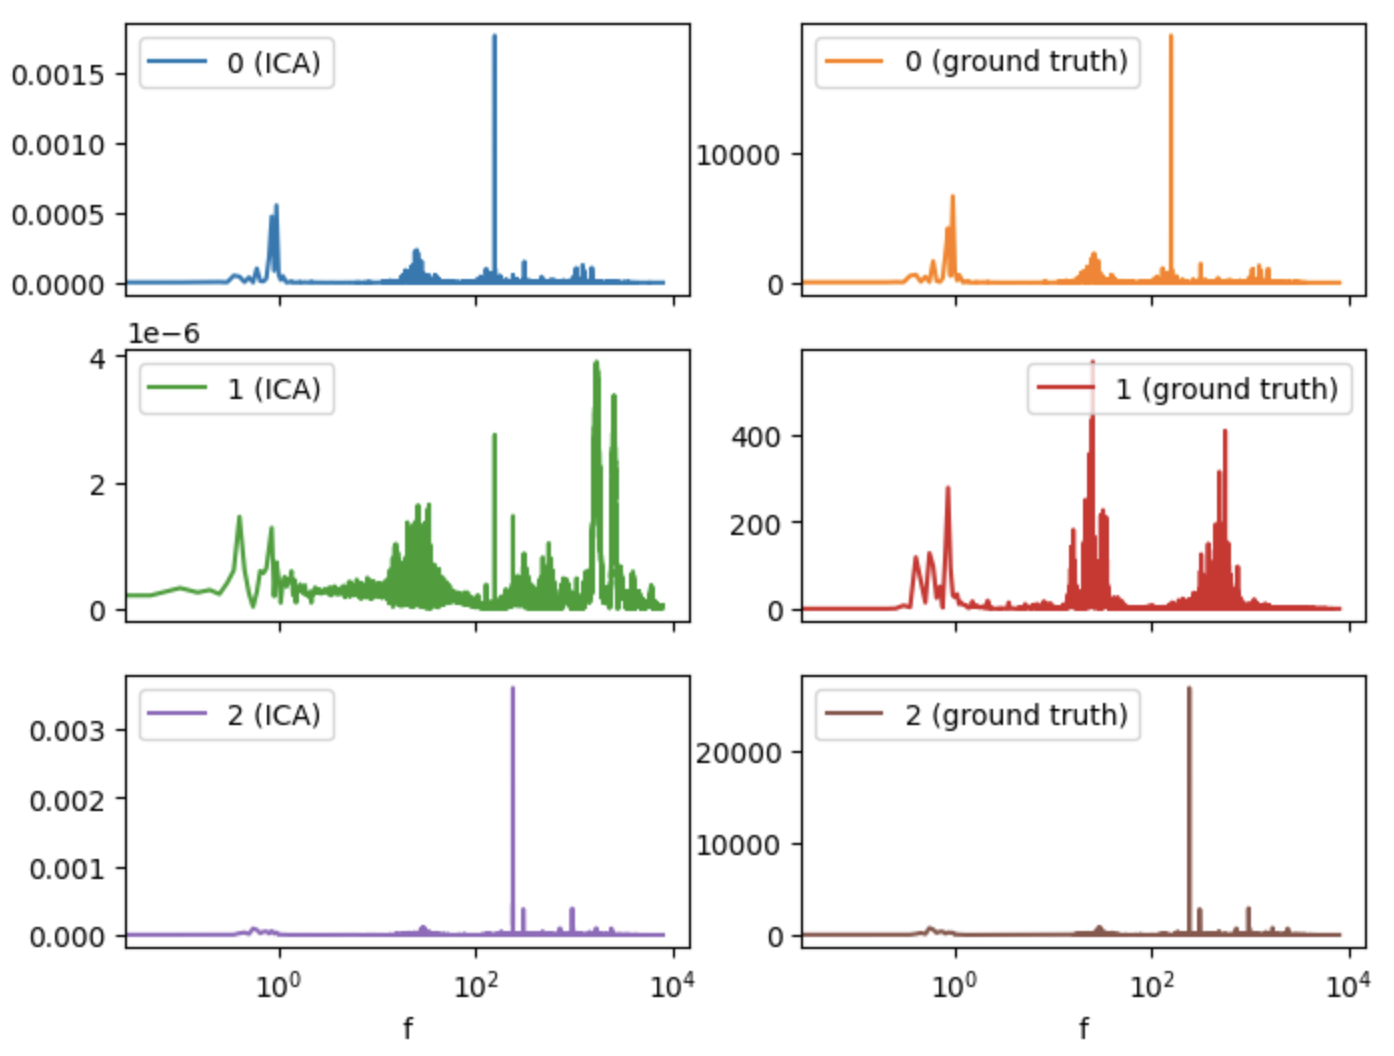
\includegraphics[width=\textwidth]{single-sensor-ica-time-domain-phase-synchronized-without-filter-source-power-spectra-full}}
        \caption{\label{fig:single-sensor-ica-time-domain-phase-synchronized-without-filter-source-power-spectra-full}}
    \end{subfigure}

    \vspace{0.1in}
    \begin{minipage}{0.85\linewidth}
    \caption{\label{fig:single-sensor-ica-time-domain-phase-synchronized-without-filter-source-power-spectra}
        Comparison of power spectra for time-domain ICA without bandpass filtering applied
        to single-sensor, multiple-time synthetic signals constructed from source signals
        that are phase-synchronized across recording times.
        (a)~Power spectra of source signals in the passband: ICA estimates (left) and
        ground truth (right).
        (b)~Power spectra of source signals at all frequencies: ICA estimates (left)
        and ground truth (right).
    }
    \end{minipage}
\end{figure}

\begin{figure}[ht]
    \centering
    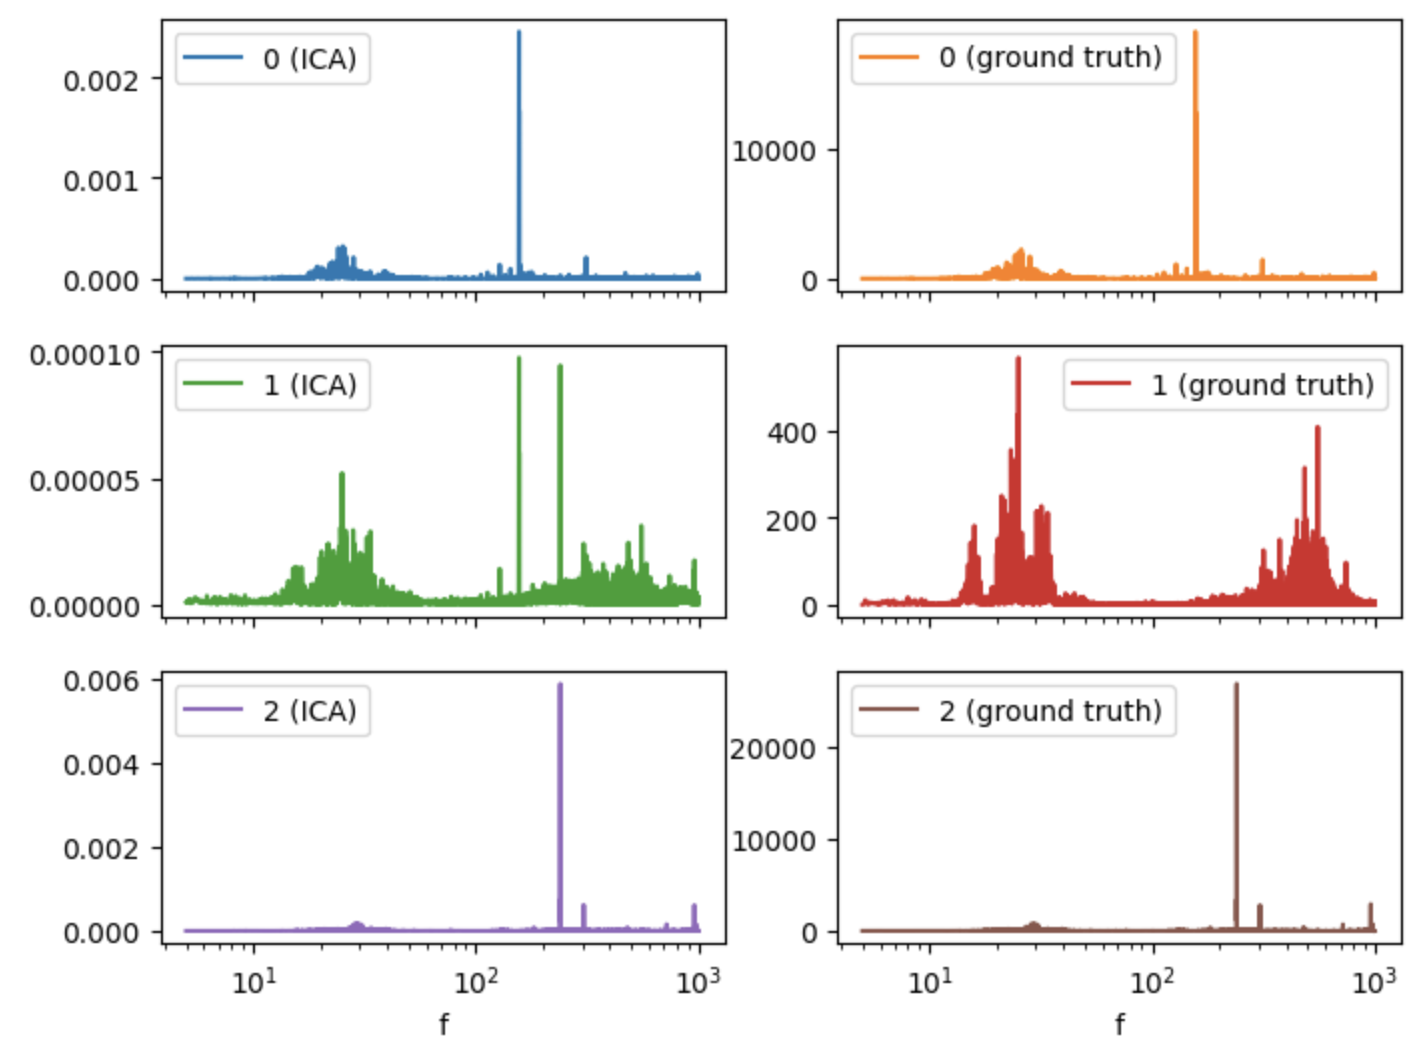
\includegraphics[width=0.5\textwidth]{single-sensor-ica-time-domain-phase-synchronized-with-filter-source-power-spectra}
    \begin{minipage}{0.85\linewidth}
    \caption{\label{fig:single-sensor-ica-time-domain-phase-synchronized-with-filter-source-power-spectra}
        Comparison of power spectra for time-domain ICA with bandpass filtering applied to
        single-sensor, multiple-time synthetic signals constructed from source signals that
        are phase-synchronized across recording times: ICA estimates (left) and ground
        truth (right).
    }
    \end{minipage}
\end{figure}

Applying a bandpass filter before performing ICA appeared to improve performance and reduce
the chance that ICA was using ambient noise to estimate signals. Visually, the power
spectra of the ICA estimated source signals appear to more cleanly match the ground truth
source power spectra. The power spectra peaks below $1$Hz appear to be difficult for ICA
to fit and may be the origin of the poorer quality source signals when bandpass filtering
is not applied.


\subsubsection*{Time-Domain ICA For Phase-Unalignd Source Signals}
For source signals that are not phase-synchronized across recording times, ICA was found to
be less effective for estimating source signals from multiple, time-separated recordings
collected using a single, stationary sensor.
Figure \ref{fig:single-sensor-ica-time-domain-phase-unaligned-without-filter-source-power-spectra}
compares the power spectrum of the estimated and ground truth source signals without
bandpass filtering.
Figure~\ref{fig:single-sensor-ica-time-domain-phase-unaligned-with-filter-source-power-spectra}
compares the power spectrum of the estimated and ground truth source signals with bandpass
filtering.

\begin{figure}[ht]
    \centering
    \hspace{-0.2in}
    \begin{subfigure}{0.4\textwidth}
        \centerline{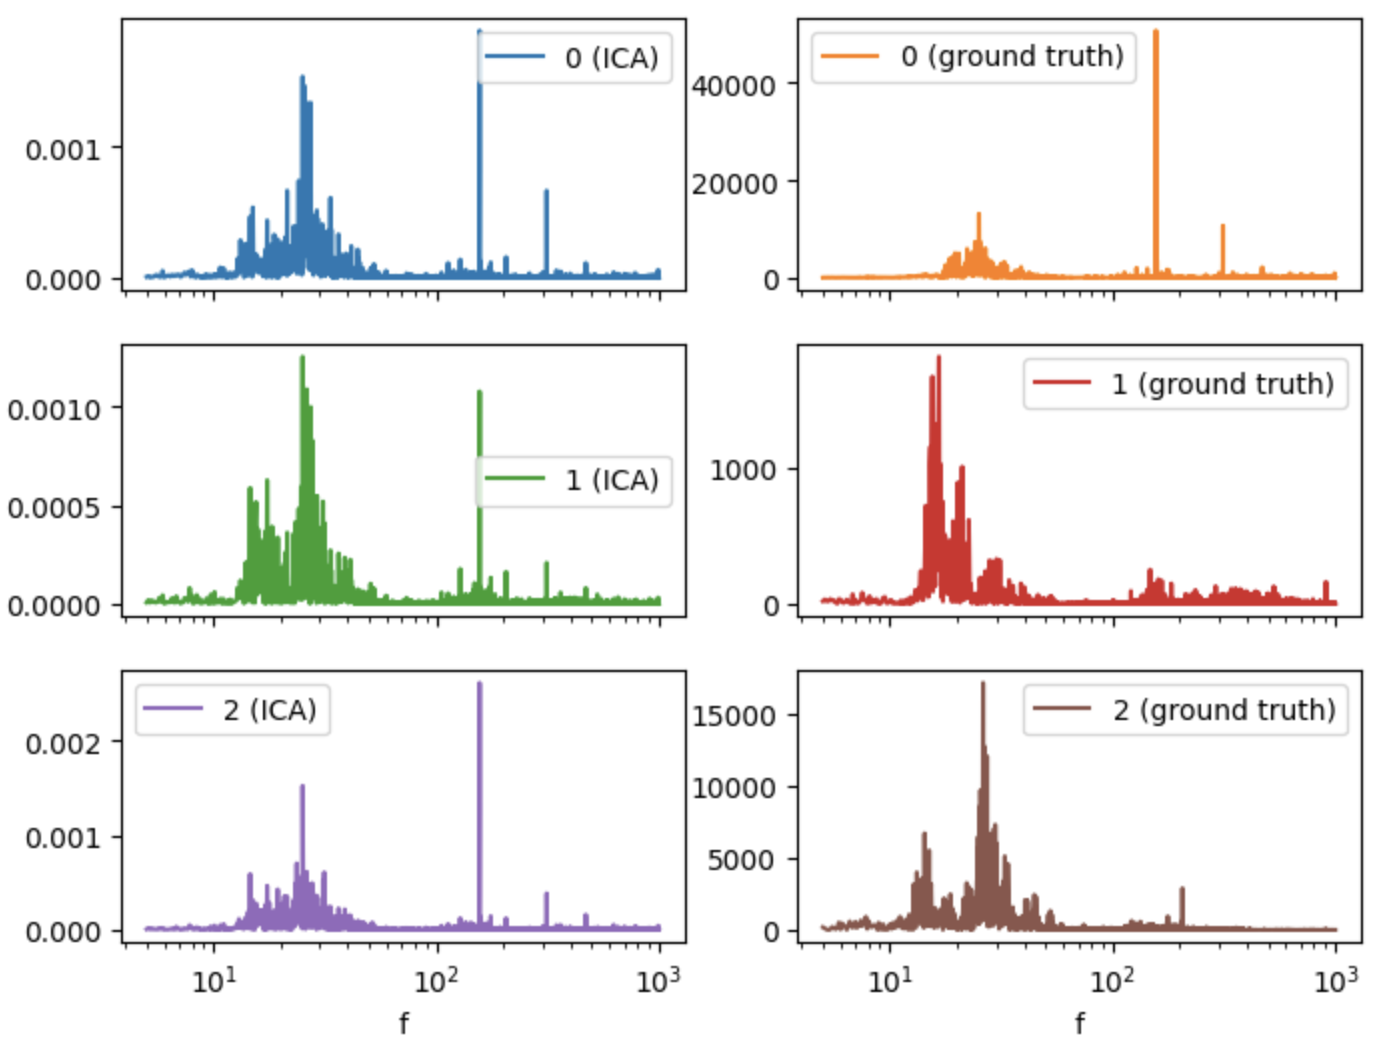
\includegraphics[width=\textwidth]{single-sensor-ica-time-domain-phase-unaligned-without-filter-source-power-spectra}}
        \caption{\label{fig:single-sensor-ica-time-domain-phase-unaligned-without-filter-source-power-spectra-passband}}
    \end{subfigure}
    \begin{subfigure}{0.4\textwidth}
        \centerline{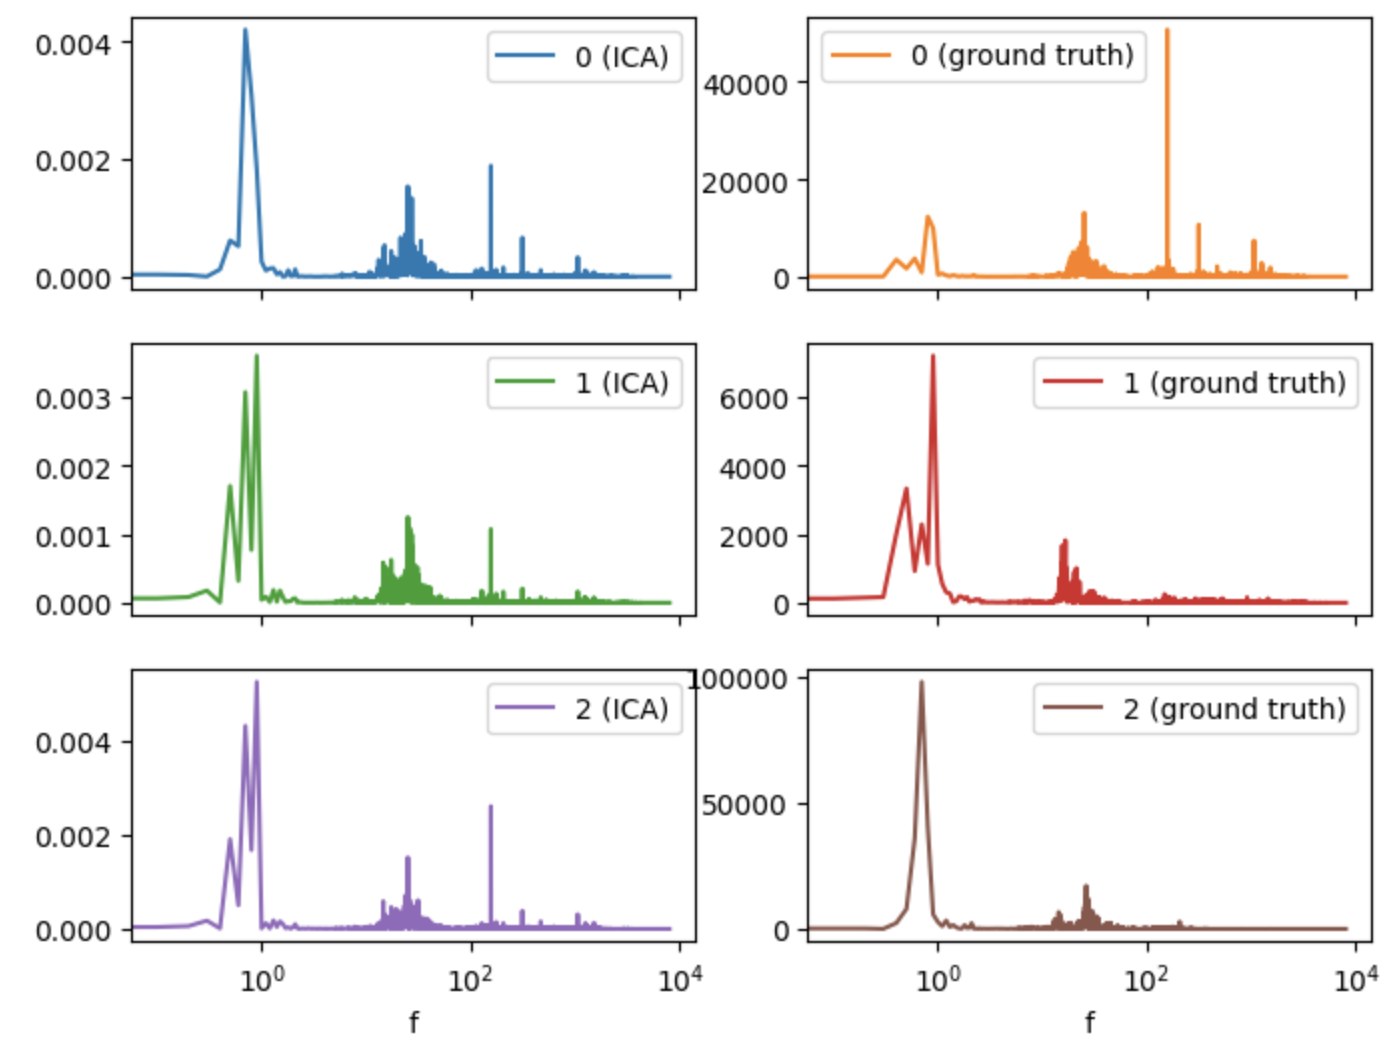
\includegraphics[width=\textwidth]{single-sensor-ica-time-domain-phase-unaligned-without-filter-source-power-spectra-full}}
        \caption{\label{fig:single-sensor-ica-time-domain-phase-unaligned-without-filter-source-power-spectra-full}}
    \end{subfigure}

    \vspace{0.1in}
    \begin{minipage}{0.85\linewidth}
    \caption{\label{fig:single-sensor-ica-time-domain-phase-unaligned-without-filter-source-power-spectra}
        Comparison of power spectra for time-domain ICA without bandpass filtering applied
        to single-sensor, multiple-time synthetic signals constructed from source signals
        that are phase-unaligned across recording times.
        (a)~Power spectra of source signals in the passband: ICA estimates (left) and
        ground truth (right).
        (b)~Power spectra of source signals at all frequencies: ICA estimates (left)
        and ground truth (right).
    }
    \end{minipage}
\end{figure}

\begin{figure}[ht]
    \centering
    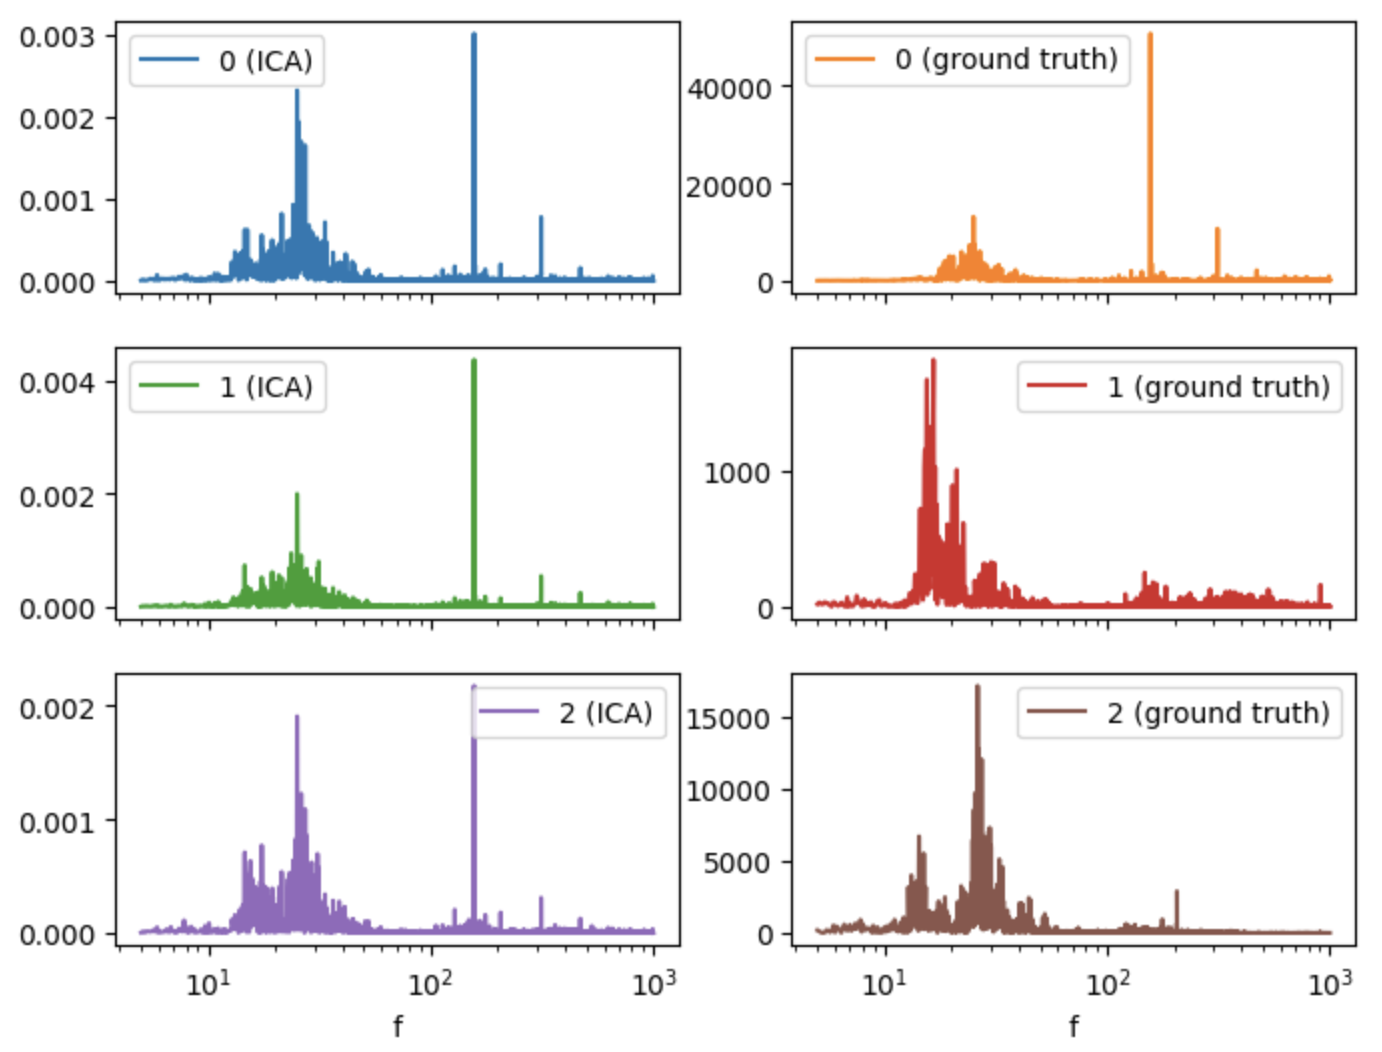
\includegraphics[width=0.5\textwidth]{single-sensor-ica-time-domain-phase-unaligned-with-filter-source-power-spectra}
    \begin{minipage}{0.85\linewidth}
    \caption{\label{fig:single-sensor-ica-time-domain-phase-unaligned-with-filter-source-power-spectra}}
        Comparison of power spectra for time-domain ICA with bandpass filtering applied to
        single-sensor, multiple-time synthetic signals constructed from source signals that
        are phase-unaligned across recording times: ICA estimates (left) and ground truth
        (right).
    \end{minipage}
\end{figure}

Applying a bandpass filter before performing ICA did not appear to significantly affect
performance. In both cases, ICA appears to be able to estimate some sources reasonably
well, but does a poorer job for other sources. The origin of the discrepancy in the quality
of source signal estimates might be the level relative phase-synchronization between
sources across recording times. ICA might be able to estimate the source signals for the
subset of source signals that are cloesest to being phase-synchronized. Source signals
less phase-synchronized might be less well estimated. These results are consistent with
the theoretical expectations for ICA.


\subsubsection*{Frequency-Domain ICA for Phase-Unalignd Source Signals}
For source signals that are not phase-synchronized across recording times, we were only
able to perform experiments applying ICA to the DFT of the mixed signals using a sine and
cosine basis because the FastICA implementation in \code{scikit-learn} is currently unable
to handle complex-valued datasets.
Figure~\ref{fig:single-sensor-ica-freq-domain-phase-unaligned-without-filter-source-power-spectra}
compares the power spectrum of the estimated and ground truth source signals without
bandpass filtering.
Figure~\ref{fig:single-sensor-ica-freq-domain-phase-unaligned-with-filter-source-power-spectra}
compares the power spectrum of the estimated and ground truth source signals with bandpass
filtering.

\begin{figure}[ht]
    \centering
    \hspace{-0.2in}
    \begin{subfigure}{0.4\textwidth}
        \centerline{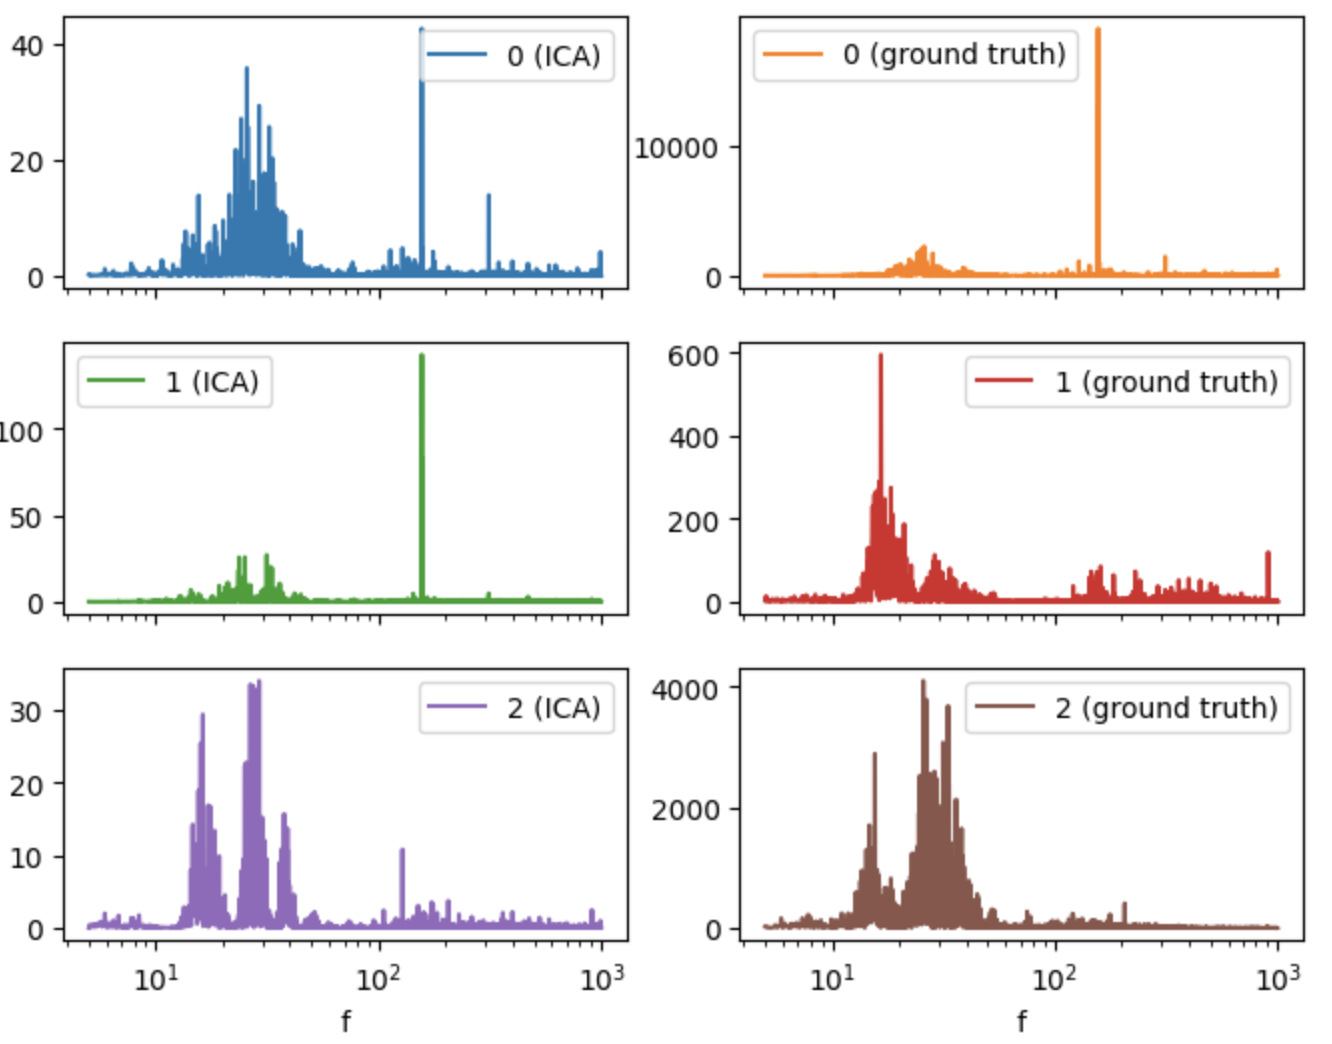
\includegraphics[width=\textwidth]{single-sensor-ica-freq-domain-phase-unaligned-without-filter-source-power-spectra}}
        \caption{\label{fig:single-sensor-ica-freq-domain-phase-unaligned-without-filter-source-power-spectra-passband}}
    \end{subfigure}
    \begin{subfigure}{0.4\textwidth}
        \centerline{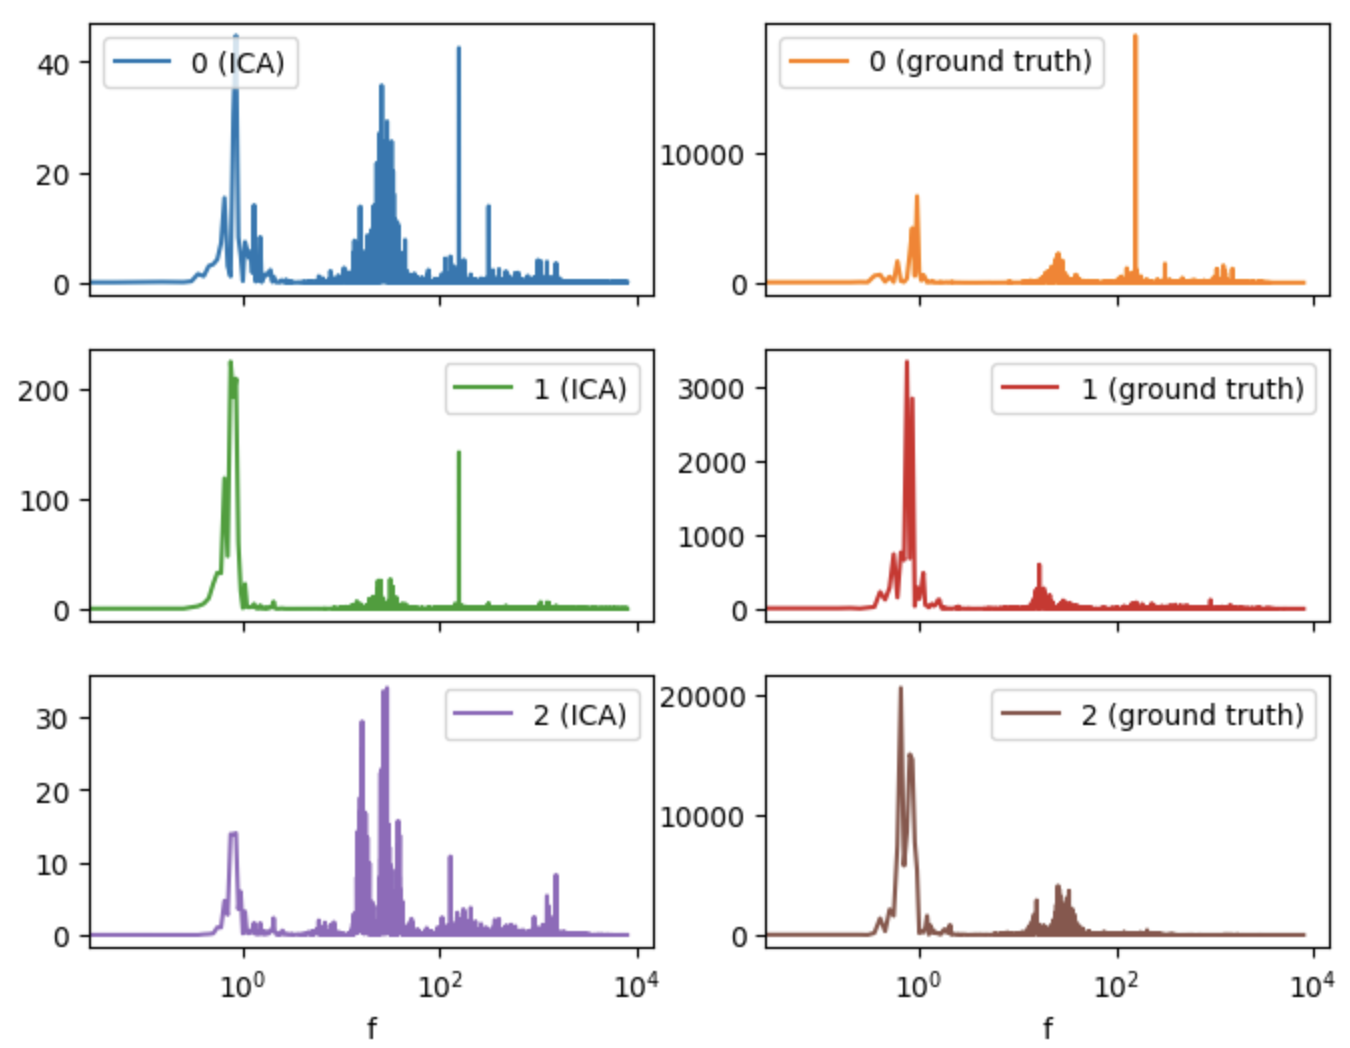
\includegraphics[width=\textwidth]{single-sensor-ica-freq-domain-phase-unaligned-without-filter-source-power-spectra-full}}
        \caption{\label{fig:single-sensor-ica-freq-domain-phase-unaligned-without-filter-source-power-spectra-full}}
    \end{subfigure}

    \vspace{0.1in}
    \begin{minipage}{0.85\linewidth}
    \caption{\label{fig:single-sensor-ica-freq-domain-phase-unaligned-without-filter-source-power-spectra}
        Comparison of power spectra for frequency-domain ICA without bandpass filtering
        applied to single-sensor, multiple-time synthetic signals constructed from source
        signals that are phase-unaligned across recording times.
        (a)~Power spectra of source signals in the passband: ICA estimates (left) and
        ground truth (right).
        (b)~Power spectra of source signals at all frequencies: ICA estimates (left)
        and ground truth (right).
    }
    \end{minipage}
\end{figure}

\begin{figure}[ht]
    \centering
    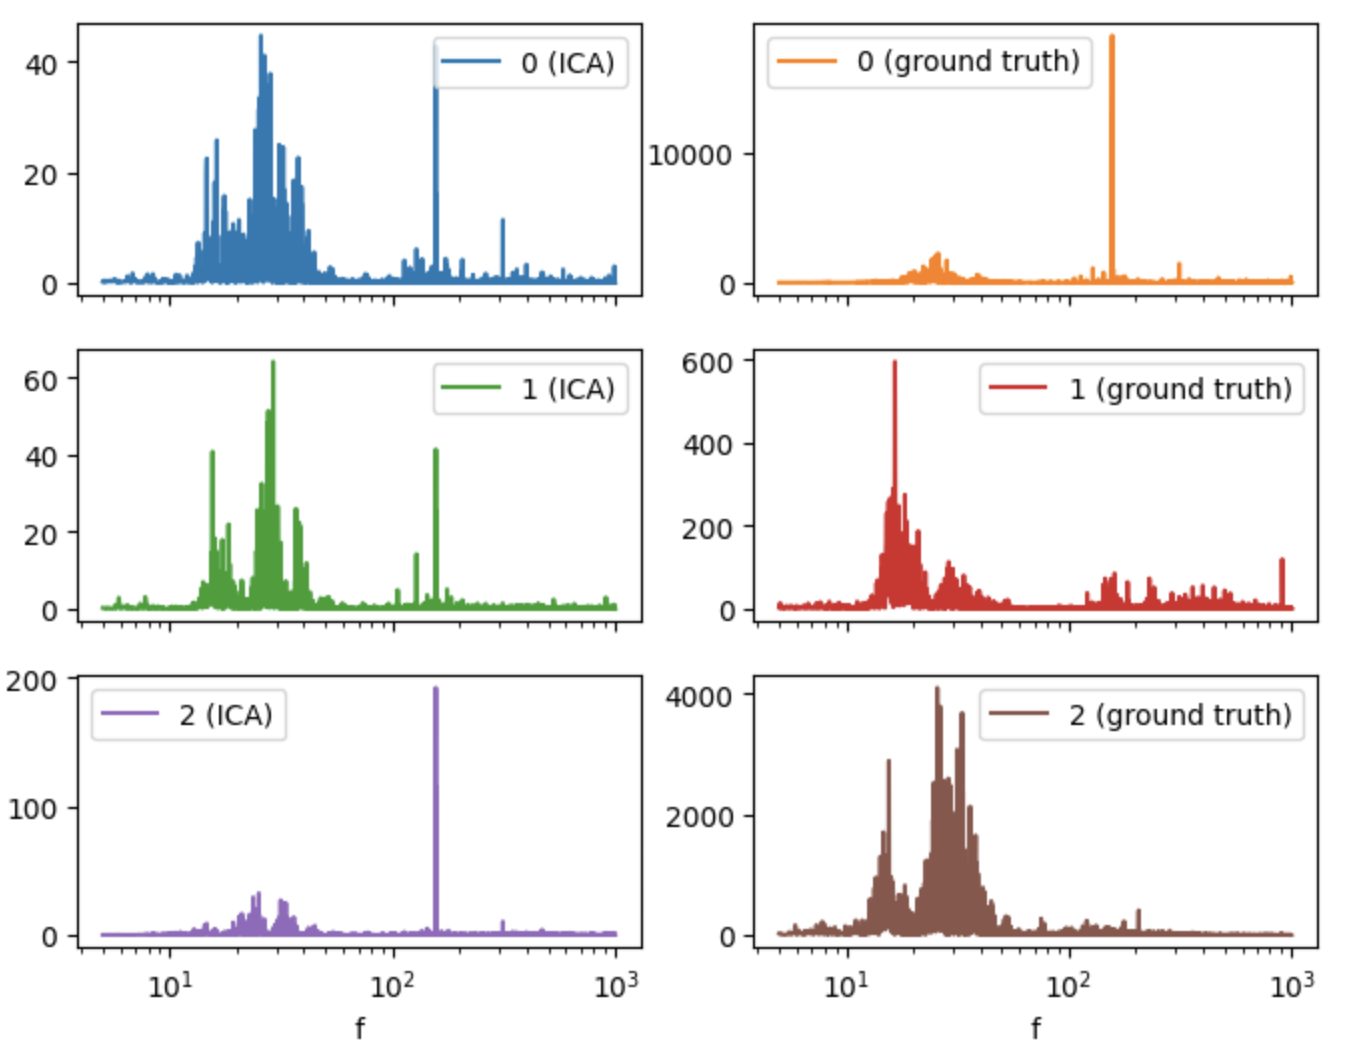
\includegraphics[width=0.5\textwidth]{single-sensor-ica-freq-domain-phase-unaligned-with-filter-source-power-spectra}
    \begin{minipage}{0.85\linewidth}
    \caption{\label{fig:single-sensor-ica-freq-domain-phase-unaligned-with-filter-source-power-spectra}}
        Comparison of power spectra for frequency-domain ICA with bandpass filtering
        applied to single-sensor, multiple-time synthetic signals constructed from source
        signals that are phase-unaligned across recording times: ICA estimates (left) and
        ground truth (right).
    \end{minipage}
\end{figure}

As expected from theory, ICA applied to the DFT with a sine and cosine basis did not
perform particularly well. Visual inspection of the power spectra indicates that the
estimated source signals contained mixtures of the ground truth source signals. Bandpass
filtering did not significantly increase the quality of the estimated source signals.

\emph{Unfortunately, the most promising approach based on application of ICA to the DFT
of the mixed signals} using a complex exponential basis \emph{could not be evaluated due to
restriction of the} \code{scikit-learn} \emph{FastICA implementation to real-valued data}.
While a few ICA implementations for complex-valued data were found, none were deemed mature
enough for this investigation (\eg, performance was too slow to be useful, it was unclear
if the code had been sufficiently debugged, \etc).  Should a suitable implementation of
ICA for complex-valued data become available in the future, this approach would be very
interesting to further investigate and explore.


\section{Summary and Conclusions}
In this report, we presented ICA-based approaches to source separation for single-sensor
systems with moving sources by leveraging the physics of acoustic waves and the
quasi-periodic nature of the source signals of interest. Using computational experiments,
we evaluated the approaches on synthetic data constructed from pure source recordings and
found ICA performance to be consistent with theoretical expectations.

\subsection*{Summary of ICA-based Source Separation Approaches and Results}
\begin{itemize}
    \item Time-domain ICA. Good source separation is achieved when source signals are
        phase-synchronized across recording times. When source signals are phase-unaligned
        across recording times, source separation is less effective.

    \item Frequency-domain ICA with sine and cosine basis. This approach is not suitable
        for phase-unaligned recording times because the relative phase shifts in the
        source signals lead to coefficient mixing, which is inconsistent with the ICA
        signal model. Computational experiments confirm that source separation is not
        particularly effective for this approach.

    \item Frequency-domain ICA with complex exponential basis. This is the most promising
        approach for source separation when source signals are phase-unaligned between
        recording times because (1) the frequency-domain signal model is consistent with
        the ICA signal model and (2) the relative phase shifts manifest as multiplicative
        changes to the mixing coefficients. Unfortunately, it was not possible to perform
        computational experiments to evaluate this approach because the \code{scikit-learn}
        FastICA implementation is limited to real-valued data.
\end{itemize}

\subsection*{Future Directions}
\begin{itemize}
    \item To assess the robustness of time-domain ICA, it would be beneficial to perform
        time-domain ICA on a wider range of synthetic datasets constructed over a wider
        range of vessel types, combinations, and number.

    \item Since time-domain ICA for phase-synchronized source signals showed good
        performance on synthetic datasets, it would be useful to perform experiments
        on non-synthetic datasets containing multiple vessels to determine whether or not
        it is reasonable to assume that real-world source signals are phase-synchronized.
        If so, time-domain ICA may be sufficient for feature engineering purposes.

    \item To assess the viability of frequency-domain ICA using a complex exponential
        basis, it would be interesting to implement ICA for complex signals. Complex-valued
        ICA algorithms have been described in the
        literature~\cite{novey:2006,novey:2007,novey:2008,novey:2008b}, but they do not
        appear to have been ported to Python.

    \item Recent research in the literature suggest that it may be possible to perform
        source separation directly on the power spectra~\cite{fu:2016}. This possibility
        would, in principle, completely eliminate issues related to phase synchronization
        of source signals and may be interesting to further investigate.
\end{itemize}

\printbibliography

\end{document}
